\question (哈尔滨工业大学,2001年)在一棵三元树中度为3的结点数为2个,度为2的结点数为1个,度为1的结点数为2个,则度为0的结点数为(
)个
\par\twoch{4}{5}{\textcolor{red}{6}}{7}
\begin{solution}在一棵度为m的树种,度为1的结点数为n1,度为2的结点数为n2,\ldots{},度为m的结点数为nm,则叶子结点数n0=1+n2+2n3+\ldots{}+(m-1)nm。
本题n0=1+1+2*2=6。
\end{solution}
\question (重庆大学,2005年)设二叉树中有n2个度为2的结点,有n1个度为1的结点,有n0个度为0的结点,则该二叉树中空指针个数为(
)
\par\twoch{n2+n1+n0}{n2+n1+2n0}{2n2+n1}{\textcolor{red}{n1+2n0}}
\begin{solution}方法一:每一个度为1的结点有1个空指针,每一个度为0的结点有2个空指针,度为2的结点没有空指针,因此结果为n1+2n0。
方法二:n个结点的二叉树有n+1个空指针,因此就有n2+n1+n0+1个空指针,又因n2=n0-1,因此共有n0-1+n1+n0+1=n1+2n0个空指针。
\end{solution}
\question (南京林业大学,2004年)按照二叉树的定义,具有3个结点的二叉树有( )种
\par\twoch{3}{4}{\textcolor{red}{5}}{6}
\begin{solution}二叉树的性质:给定n个结点,能构成种不同的二叉树。这里n=3,答案为5,因此本题选C。
\end{solution}
\question (西南交通大学,2005年)若某完全二叉树的结点个数为100,则第60个结点的度为(
)
\par\twoch{\textcolor{red}{0}}{1}{2}{不确定}
\begin{solution}完全二叉树的结点个数为偶数,说明有1个度为1的结点。
设ni为度是i的结点的个数,那么就有n0+n2+1=100,n0=n2+1,解得n0=55,n2=54。
又因完全二叉树的编号,是先度为2的结点,然后度为1的结点,最后才是叶子结点。
即1~54是度为2的结点,55是度为1的结点,56~100是度为0的结点。本题问的是第60个结点,因此是度为0的结点。
\end{solution}
\question (北京航空航天大学,2000年)具有10个叶结点的二叉树中有( )个度为2的结点
\par\twoch{8}{\textcolor{red}{9}}{10}{11}
\begin{solution}设ni为度是i的结点的个数,n0=1+n2,得到n2=n0-1=10-1=9。
\end{solution}
\question (西安交通大学,1996年)一棵完全二叉树上有1001个结点,其中叶子结点的个数是(
)
\par\twoch{250}{500}{254}{\textcolor{red}{以上都不正确}}
\begin{solution}完全二叉树,度为1的结点,要么是0个,要么是1个。如果总结点数是奇数(偶数),则度为1的结点数是0(1)个。
本题总结点数就是个奇数,因此度为1的结点数是0个。
设ni为度是i的结点的个数,那么
n0+n2=1001,又有n0=1+n2,解得:n0=501,n2==500。
\end{solution}
\question (南京理工大学,1999年)当一棵有n个结点的二叉树按层次从上到下,同层次从左到右将数据存放在一维数组A{[}1\ldots{}n{]}中时,数组中第i个结点的左孩子为(
)
\par\twoch{A[2i](2i≤n)}{A[2i+1](2i+1≤n)}{A[i/2]}{\textcolor{red}{无法确定}}
\begin{solution}只有完全二叉树可以确定左孩子为A{[}2i{]}(2i≤n),而本题并未说明是完全二叉树,因此是无法确定。
\end{solution}
\question (北京航空航天大学,2003年)若一棵深度为6的完全二叉树的第6层有3个叶子结点,则该二叉树共有(
)个叶子结点
\par\twoch{\textcolor{red}{17}}{18}{19}{20}
\begin{solution}先计算第5层的结点数:24=16个结点。又第6层3个结点把第5层的2个结点占用了,故第5层的叶结点为16-2=14,又第6层有3个叶结点,总共就有14+3=17个叶结点。
\end{solution}
\question (北京理工大学,2001年)二叉树的第i层上最多含有结点数为( )
\par\fourch{}{}{\textcolor{red}{}}{}
\begin{solution}第1层为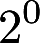
\includegraphics[width=0.14583in,height=0.15625in]{texmath/2f67ff5Cdpi7B3507D25E0},第2层为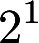
\includegraphics[width=0.14583in,height=0.15625in]{texmath/3177ee5Cdpi7B3507D25E1},第i层为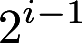
\includegraphics[width=0.30208in,height=0.15625in]{texmath/4c66015Cdpi7B3507D25E7Bi-17D}。
\end{solution}
\question (华南理工大学,2005年)一棵深度为4的完全二叉树,最少有( )个结点
\par\twoch{4}{\textcolor{red}{8}}{15}{6}
\begin{solution}深度为3的满二叉树的结点数为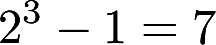
\includegraphics[width=0.78125in,height=0.16667in]{texmath/1f3b305Cdpi7B3507D25E3-13D7},再加一个结点就成为深度为4的最少结点的完全二叉树了,即结点为8。
【总结】深度(高度)是n的完全二叉树,最多结点是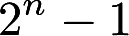
\includegraphics[width=0.46875in,height=0.13542in]{texmath/9438eb5Cdpi7B3507D25En-1}个,最少是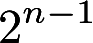
\includegraphics[width=0.33333in,height=0.15625in]{texmath/1dcd255Cdpi7B3507D25E7Bn-17D}个。
\end{solution}
\question (北京邮电大学,2007年)一棵深度为7的满二叉树共有( )个非终端结点
\par\twoch{31}{\textcolor{red}{63}}{127}{255}
\begin{solution}解法一:
深度为7的满二叉树的结点数为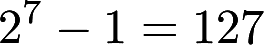
\includegraphics[width=0.94792in,height=0.16667in]{texmath/dd04ad5Cdpi7B3507D25E7-13D127}。
设
\includegraphics[width=0.13542in,height=0.11458in]{texmath/fc7cb75Cdpi7B3507D7B7B5Crm7Bn7D7D_7B5Crm7Bi7D7D7D}为度是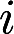
\includegraphics[width=0.05208in,height=0.11458in]{texmath/2a80255Cdpi7B3507Di}的结点的个数,则有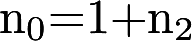
\includegraphics[width=0.68750in,height=0.14583in]{texmath/55ffa05Cdpi7B3507D7B7B5Crm7Bn7D7D_07D7B5Crm7B3D7D7D17B5Crm7B2B7D7D7B7B5Crm7Bn7D7D_27D},又因满二叉树没有度为1的结点,因此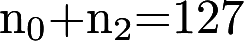
\includegraphics[width=0.87500in,height=0.15625in]{texmath/85230f5Cdpi7B3507D7B7B5Crm7Bn7D7D_07D7B5Crm7B2B7D7D7B7B5Crm7Bn7D7D_27D7B5Crm7B3D7D7D127},解得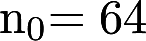
\includegraphics[width=0.52083in,height=0.14583in]{texmath/3e62be5Cdpi7B3507D7B7B5Crm7Bn7D7D_07D7B5Crm7B3D647D7D},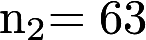
\includegraphics[width=0.52083in,height=0.14583in]{texmath/c4bc875Cdpi7B3507D7B7B5Crm7Bn7D7D_27D7B5Crm7B3D637D7D},本题的非终端结点数就是度为2的结点,即为63。
解法二:
深度为7的满二叉树,除去最后一层叶结点,即都为非终端结点,其实就是深度为6的满二叉树,因此非终端结点数目=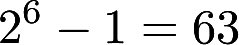
\includegraphics[width=0.85417in,height=0.16667in]{texmath/076ca35Cdpi7B3507D25E6-13D63},本题选B。
\end{solution}
\question (华南理工大学,2006年)以下说法中正确的是( )
\par\fourch{\textcolor{red}{完全二叉树中,叶结点的双亲的左兄弟(如果存在)一定不是叶结点}}{任何一棵二叉树,终端结点数等于度为2的结点数减1}{二叉树不适合用顺序结构存储}{结点按层次序编号的二叉树,第i个结点的左孩子(如果存在)的编号为2i}
\begin{solution}A正确,叶结点的双亲的左兄弟(如果存在)必然是度为2的结点,不可能是叶结点。
B错误,不是减1而是加1。可以假设一个只有根结点的二叉树,终端为1,不符合B选项的描述。
C错误,完全二叉树很适合顺序存储。
D错误,这个是完全二叉树的性质。可考虑单支树进行排除。
\end{solution}
\question (北京航空航天大学,2002年)已知某完全二叉树采用顺序存储结构,结点数据信息的存放顺序依次为ABCDEFGH,该完全二叉树的后序遍历序列为(
)
\par\twoch{\textcolor{red}{HDEBFGCA}}{HEDBFGCA}{HDEBAFGC}{HDEFGBCA}
\begin{solution}画出该完全二叉树的示意图(下图)后,易得其后序遍历序列为HDEBFGCA,故本题选A。
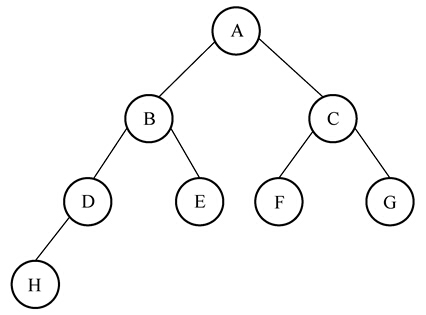
\includegraphics[width=2.08333in,height=2.08333in]{computerassets/82999f59b924ff27710fe8094367a64b.jpeg}
\end{solution}
\question 已知一棵完全二叉树的第6层(设根为第1层)有8个叶结点,则该完全二叉树的结点个数最多是(
)
\par\twoch{39}{52}{\textcolor{red}{111}}{119}
\begin{solution}完全二叉树的叶子结点只可能在完全二叉树最后(最深)两层,也就是说第6层可能是最后一层(共有6层),也可能是倒数第二层(共有7层)。明显,结点最多的情况是后者,即1~6层构成一个满二叉树,1~6满二叉树的结点总数为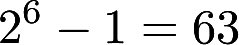
\includegraphics[width=0.85417in,height=0.16667in]{texmath/076ca35Cdpi7B3507D25E6-13D63}。
现在需要求的是第7层的结点数目,因为第6层有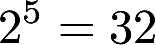
\includegraphics[width=0.56250in,height=0.15625in]{texmath/54f3d45Cdpi7B3507D25E53D32}个结点,这32个结点中有8个叶子结点,也就是有32-8=24个非叶子结点,这些非叶子结点每个最多有两个孩子结点,共计48个叶子结点。
这样最多的结点总个数=6层满二叉树结点数+第7层结点数=63+48=111。
\end{solution}
\question 已知一棵有2011个结点的树,其叶结点个数为116,该树对应的二叉树中无右孩子的结点的个数是(
)
\par\twoch{115}{116}{1895}{\textcolor{red}{1896}}
\begin{solution}解法一: 可以采用特殊情况法去解。可举以下特例:
如下图所示,则对应的二叉树中仅有最后115个结点有右孩子。
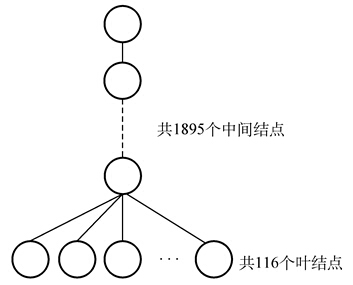
\includegraphics[width=3.67708in,height=2.96875in]{computerassets/15743e12ab14bbeb49ea10ccba83edeb.jpeg}
解法二:
设一棵二叉树是由森林转换而来的,若森林中有n个非终端结点,则二叉树中无右孩子的结点个数为n+1。证明如下:
因为森林中的非终端结点,转换为二叉树后,其孩子都在其左子树的右链中,其末端一定有一个无右孩子的结点。加上跟结点本身,转换为二叉树后也没有右孩子,故二叉树中无右孩子的结点个数为n+1。
每个非终端结点转换成二叉树后都对应一个无右孩子的结点(因为一个非终端结点至少有一个孩子结点,其最右边的孩子结点转换成二叉树后一定没有右孩子),另外,最后一棵树的根结点转换成二叉树也没有右孩子。
本题中非终端结点个数=2011-116=1895,因此二叉树中无右孩子的结点个数=1895+1=
1896。 【总结】 ① 相比于解法二,解法一更快速和直观。 ②
当森林、树转换成对应的二叉树后,结点的左链是原孩子关系,右链是原兄弟关系。
\end{solution}
\question (北京航空航天大学,2004年)若一棵二叉树有1001个节点,且无度为1的节点,则叶节点的个数为(
)
\par\twoch{498}{499}{500}{\textcolor{red}{501}}
\begin{solution}设叶子节点的个数为x,则有(1001-x)*2+1=1001,解得为501
\end{solution}
\question (上海交通大学,2005年)树中所有节点的度等于所有节点数加( )
\par\twoch{0}{1}{\textcolor{red}{-1}}{2}
\begin{solution}若树中只有根节点,则度为0,节点数为1;每添加一个节点,则节点数加1,所有节点的度也加1;故树中所有节点的度等于所有节点数减1
\end{solution}
\question (南京理工大学,2004年)一颗有64个叶子节点的完全二叉树,该完全二叉树最多有(
)节点
\par\twoch{124}{125}{126}{\textcolor{red}{127}}
\begin{solution}完全二叉树最多节点就是满树的情况
\end{solution}
\question (上海交通大学,2005年)在一棵具有n个节点的二叉树中,所有节点的空子树的个数等于(
)
\par\twoch{n}{n-1}{\textcolor{red}{n+1}}{2*n}
\begin{solution}一个简单的方法是将所有的空链域看成一棵子树,这样,原来所有的节点都是双分支节点,根据叶子节点数=双分支节点数+1,此时这里的叶子节点是原来的空链域,即n+1
\end{solution}
\question (中南大学,2005年)有n个节点的完全二叉树采用顺序存储结构,从根节点开始对其层次顺序进行编号(设根结点编号为1),下列说法错误的是(
)
\par\fourch{当1≤i≤n/2,节点i的左子女是节点2i,否则节点i没有左子女}{当1≤i≤(n-1)/2时,节点i的右子女是节点2i+1,否则节点i没有右子女}{\textcolor{red}{1≤i≤n时,节点i的父母节点是i/2(向下取整)}}{当i为偶数且1≤i≤n时,节点i的父母节点是i/2}
\begin{solution}对于C选项,如果i=1,则根节点的父母节点为0,而根节点没有父母节点,所以错误
\end{solution}
\question (南京邮电大学,2005年)一棵三叉树中,已知度为3的节点个数等于度为2的结点数,且树中叶子节点的数目为13,则度为2的节点数目为(
)
\par\twoch{\textcolor{red}{4}}{2}{3}{5}
\begin{solution}首先,我们必须知道总结点数=分支数+1,假设度为3的节点有x个,度为2的节点有y个,度为1的节点有z个,度为0的节点有m个,那么有x+y+z+m=3x+2y+z+1,将m=13,x=y代入,可得x=4。
\end{solution}
\question (中国矿业大学,2004年)二叉树有10个度为2的节点,5个度为1的节点,叶节点数为(
)
\par\twoch{10}{9}{\textcolor{red}{11}}{不确定}
\begin{solution}根据叶子节点数=双分支节点数+1得叶子节点数为11
\end{solution}
\question (重庆大学,2004年)一颗有124个叶子的完全二叉树,最多有( )个节点
\par\twoch{247}{\textcolor{red}{248}}{249}{250}
\begin{solution}因为124个叶子节点,故双分支节点个数为123,另外由于是完全二叉树,单分支节点数最多只可能为1,故总结点不会超过124+123+1=248.排除C、D。因为叶子节点数为124,故叶子节点一定集中在第7层和第8层,若第8层排满会有128个节点,每去除最后一层两个兄弟节点,总叶子节点数减1(上层增加一个,下层减少两个),可知最后一层最多有121个节点,所以最多有127+121=248个节点
\end{solution}
